\section{GameBank}

In this section we will illustrate the notable features of GameBank. Since 
describing all the design choices made during the application development would 
result in a long explanation, we invite the reader to take a look at the public 
repository available in~\cite{gamebank18}.

\subsection{How it works}

GameBank, as already described in Section CHANGEME, \todo{Section 1 ref 
missing} is an application complementary to a board game. It helps players 
removing some burden related to manage possible in-game transaction, 
distributing the task to the members and eliminating the need of a game master.

Since the social nature of board games, the application is designed to work 
in multiplayer-only mode. Indeed, because a single player match is a particular 
instance of a multiplayer game, the application can start a match even with one 
member, but it has to keep the Bluetooth link on.

The application allows users to customize their profile in the settings 
activity, where they can change username or profile picture. If the profile is 
not set when a match is starting, a new one is randomly generated. The master 
in order to recognize players in a match it uses a UUID (Universally Unique 
Identifier), so different players can have the same username.

There are two ways to start a match: loading the game from a save and starting 
a new one. In any case, the smartphone performing one of these actions becomes 
the Bluetooth master, and it starts waiting for other players to join the 
lobby. When a player joins, she has the possibility to ``poke'' the master, 
that sees a toast message on her screen. Additionally, the player that join the 
match has to set herself as ready: indeed a match can not start if anyone in the 
lobby is not ready. 
The connections created is an ad-hoc one, but as a matter of fact the master 
forwards the packets it receives to everyone after the match starts, simulating 
a P2P (Peer-to-Peer) networking. We saw this as an opportunity to semplificate 
transaction communications.
When all the conditions to start the match are met, the host has the 
possibility start it, making every conncted devices display the dashboard 
activity.

The dashboard activity is subdivided in two tabs: one for transfer money and 
the other one to see the transaction log. In the first tab, users can send 
money to each other or to themselves (impresonating the bank). In the second 
tab, there is the transaction log, that is updated every time someone creates a 
new transaction. In this log, players can see all the transactions. In this 
way, they can check if someone is cheating. \todo{Here we should put a 
screenshot of the application}

\subsection{Architecture}

GameBank architecture is composed of two layers \todo{Insert figure here}: one 
for the communications/networking and the other one for the game logic. With 
this architecture data trasmission and game logic are highly decoupled, so that 
is easy to make changes to one of the two parts. In particular, this could lead 
to a simpler re-utilization of the network layer in other applications.

The whole application is built using the event architecture. Every change in 
the application state is interpreted as a new event, that has a particular tag 
and is captured from subscribers along the application. While this seems to 
make the flow difficult to understand and cubersome, it actually allows to keep 
the code very decoupled.

Regarding the network layer, it is built in a way that host and client 
operations are as similar as possible. The only different parts are the way 
clients and hosts get the MAC address of the receiver. In particular, the host 
has to keep in memory all the clients addresses, while the clients need to 
keep in memory only the host address. A particular object, \texttt{BTBundle} is 
used as a wrapper where other layers can put data to send.

\begin{figure}[t]
 \centering
 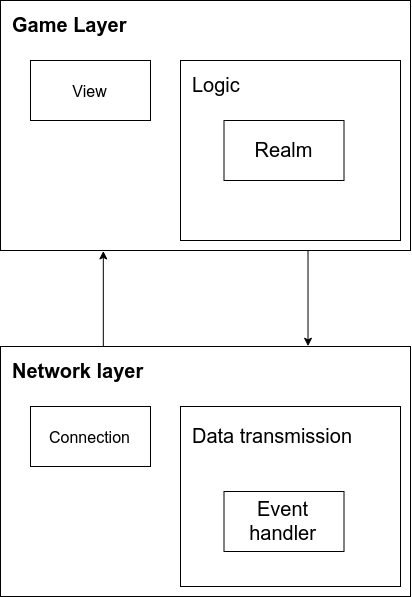
\includegraphics[scale=0.4]{GameBank}
 \caption{GameBank architecture}
 \label{fig:gbArchitecture}
\end{figure}

The game layer simply takes the events coming from the network transmissions, 
and store the data in a Realm database\footnote{\url{https://realm.io/}}, that 
is based on events too. Finally, the views get updated with new data stored in 
the database.
